\documentclass{jdf}

\begin{document}
Section: PUBP-6727
\title{Mutual Monitoring in the Cloud \\ Progress Report 4}
\author{Alexander Stein}

\maketitle
\thispagestyle{fancy}


\section*{Problem Statement}

Cloud computing infrastructure is essentially ubiquitous, but adoption is not without challenges. Cloud service providers must cater to customers in regulated sectors, complying with cybersecurity frameworks that create high barriers to entry. One barrier is ongoing evaluation of the provider's cybersecurity posture, often resulting in centralized bureaucracies. FedRAMP oversees a prominent example of such a program, the Continuous Monitoring Program, which is emblematic of these barriers. This program requires hundreds of cloud service providers to contract with one of thirty reputable auditor firms. The providers work with the auditors to send security scans and updated security control documentation for FedRAMP-authorized services monthly to FedRAMP reviewers, in some cases for the largest cloud infrastructures in the world. All three parties collaborate in meetings, emails, and a wiki, forming a unique multi-party bureaucracy that both secures and bottlenecks the government's acquisition of modern cloud services.

Are these bureaucracies an optimal solution, or a last resort that fails to keep pace with cloud technology as it proliferates and evolves? If they are a last resort, is there a better way?

\section*{Solution Statement}

I will use this research to design and evaluate an alternative to centralized continuous monitoring, mutual monitoring. The foundation of mutual monitoring will be federated data services, known in other security use cases as \hyperlink{https://transparency.dev}{transparency services}. The positives and negatives of FedRAMP's continuous monitoring model will inform its design. Operating such services can change the economics, and thereby the behavior, of cloud service providers and their customers. A new architecture will incentivize auditors to sell value-add analytics via these federated data services, potentially obsoleting centralized authorities for continuous monitoring like FedRAMP.

\section*{Completed Tasks (Last 2 Weeks)}

\begin{enumerate}
    \item I updated the architecture specification. I am still waiting for final feedback from subject-matter experts advising me.
    \item I continued limited development of the core transparency service and utility classes shared with Relying Party clients, but I deferred further development.
    \item I finalized my critical analysis of FedRAMP, waiting for feedback from subject matter experts reviewing my solution.
    \item I further developed Monte Carlo simulations in Python and supporting data for cost and duration estimation.
    \item I developed a simple quantitative framework for measuring performance of inventory management and configuration management.
    \item For evaluating my project with qualitative methods per my plan, I coded the theme, sentiment, and persona of several hundred comments in my archive of past and current FedRAMP 20x working group feedback.
\end{enumerate}

\section*{Tasks for the Next Project Report}

In the next week, I will complete architecture, analysis, and evaluation. For the following two weeks, I will draft the final paper.

\section*{Questions or issues I'm having}

\subsection*{Deliverables and Scope}

\begin{enumerate}
    \item I intended to focus on code and accelerate development, but I deferred development to focus on developers which I am closer to completing. 
\end{enumerate}

\subsection*{Evaluation and Measurement}

\begin{enumerate}
    \item Properly designing user interview questions for interviews and scheduling are a significant challenge, just like the professors warned and I assumed. This next week will be challenging, but I look forward to it!
\end{enumerate}

\section*{Methodology Paragraph Summary}

For this project, I will use multiple methods to implement an alternative architecture for monitoring cloud services and modeling its potential impact. To start, I will use a quantitative and qualitative analysis of the current shortcomings and gaps for the current FedRAMP Continuous Monitoring Program. This will be the primary example of centralized continuous monitoring for which I design my mutual monitoring model for comparison. For qualitative analysis, I can perform textual analysis and sentiment analysis. I will leverage academic research, industry analysis, and a new primary source: FedRAMP's web-based forums for \hyperlink{https://www.fedramp.gov/20x/working-groups/}{the 20x reform initiative and its community working groups}. In these forums, stakeholders discuss their praise and criticism of current centralized processes and plans for future ones, often summarizing their pain points highly relevant to designing an alternative process. In addition, I will use publicly available information from FedRAMP and industry analysis to quantify the burden of the current FedRAMP Continuous Monitoring and its manual workflow. As I build a prototype based on my architecture, I will design several use cases to estimate the cost and resource efficiency to compare those costs against the estimated costs for my solution. In addition to these methods, I will use advisors familiar with FedRAMP from different stakeholder perspectives to validate information or analysis where these methods prove lacking and leave gaps.

\section*{Timeline}

\begin{xltabular}{\textwidth}{|l|X|l|}
    % \caption{Timeline for Mutual Monitoring Project} 
    % \label{tab:timeline} \\
    \hline \multicolumn{1}{|c|}{\textbf{Week \#}} & \multicolumn{1}{c|}{\textbf{Description of Task}} & \multicolumn{1}{c|}{\textbf{Status}} \\
    \endfirsthead
    \hline
    % \multicolumn{3}{c}%
    % {\tablename\ \thetable{} -- continued from previous page} \\
    % \hline \multicolumn{1}{|c|}{\textbf{Week \#}} & \multicolumn{1}{c|}{\textbf{Description of Task}} & \multicolumn{1}{c|}{\textbf{Status}} \\ \hline 
    % \endhead
    % \hline \multicolumn{3}{|r|}{{Continued on next page}} \\ \hline
    % \endfoot    
    % \hline
    % \endlastfoot
    W6 (June 16-22) & Complete data service client to submit to submission API instances. & Deferred \\
    \hline
    W6 & Design MVP continuous monitoring use cases and quantitative measurements. & Deferred \\
    \hline
    W6 & Implement data service client to submit to submission API instances. & Deferred \\
    \hline
    W6 & Complete data service internals and submission API. & Deferred \\
    \hline
    W6 & Build data export tool for complete, offline archive of 20x forums. & Continued \\
    \hline
    W7 (June 23-29) & Complete FedRAMP critical analysis document. & In Progress \\
    \hline
    W7 & Build data export tool for complete, offline archive of 20x forums. & Completed \\
    \hline    
    W7 & Complete implementation of data service client to submit to submission API instances. & Deferred \\
    \hline    
    W7 & Implement MVP continuous monitoring use cases in API quantitative processing module. & Deferred \\
    \hline
    W7 & Design MVP continuous monitoring use cases and quantitative measurements. & Deferred \\
    \hline
    W7 & Finalize architecture specification with advisors' reviews. & Pending \\
    \hline
    W7 & Implement continuous monitoring quantitative processing module for API. & Deferred \\
    \hline
    W7 & Recruit stakeholders to interview for project evaluation. & Completed \\
    \hline          
    W8 (June 30 - July 6) & Start prototype deployment to cloud service tenants for testing. & Pending \\
    \hline
    W8 & Design MVP continuous monitoring use cases and quantitative measurements. & Completed \\
    \hline
    W8 & Implement continuous monitoring quantitative processing module for API. & Deferred \\
    \hline    
    W8 & Interview stakeholders for project evaluation. & Deferred \\
    \hline  
    W9 (July 7-13) & Complete prototype deployment to cloud service tenants for testing. & Deferred \\
    \hline
    W9 & Interview stakeholders for project evaluation. & Pending \\
    \hline
    W9 & Complete Monte Carlo simulations and supporting activities for evaluation. & Pending \\
    W10 (July 14-21) & Tie up loose ends on project deliverables and paper. & Pending \\    
    \hline    
\end{xltabular}

\section*{Evaluation}

\documentclass{jdf}

\begin{document}
Section: PUBP-6727
\title{Mutual Monitoring in the Cloud \\ Evaluation Plan}
\author{Alexander Stein \\ \hyperlink{mailto:astein38@gatech.edu}{astein38@gatech.edu}}

\maketitle
\thispagestyle{fancy}

\section*{Summary}

The project, as \hyperlink{https://github.com/aj-stein/practicum_proposal/blob/5238ba70dd8736320400ee6907b3fcfdd8ae672b/paper.pdf}{detailed in the intial proposal}, examines the many challenges to effective multi-party security monitoring of cloud service providers and designing a solution based on two areas of work. The first area of work is an analysis of best-in-class contemporary techniques for multi-party cloud security monitoring, typified by FedRAMP's administration of their \hyperlink{https://web.archive.org/web/20250616221039/https://www.fedramp.gov/assets/resources/documents/CSP_Continuous_Monitoring_Performance_Management_Guide.pdf}{Continuous Monitoring Program}. The second area of work, informed by the first, is a specification and prototype for a novel architecture for multi-party security monitoring of cloud service providers, addressing challenges and shortcomings identified from the first work area.

To evaluate the solution, I plan to use a multi-disciplinary approach to assess the project's final deliverables, identifying benefits to the proposed solutions; confirm and discover limitations to the solution; and propose future areas of work. I categorize this multi-disciplinary approach into qualitative and quantitative methods, which I describe in more detail below.

\subsection*{Quantitative Methods}

Evaluating this project will include the quantitative methods below.

\begin{enumerate}
  \item Model the range of costs for continuous monitoring process, data access, and submission for FedRAMP's current requirements.
  \item Model the range of duration for processes related to continuous monitoring activities for FedRAMP's current requirements.
  \item Model and estimate the equivalent processes in the proposed mutual monitoring architecture.
\end{enumerate}

\subsection*{Qualitative Methods}

Evaluating this project will include the qualitative methods below.

\begin{enumerate}
  \item Identify challenges and obstacles to current FedRAMP continuous monitoring processes through resources including. but not limited to:
  \begin{itemize}
    \item literature review of multi-party security monitoring of cloud service providers, as FedRAMP and other regulatory frameworks implement it;
    \item sentiment analysis FedRAMP's official forum for its 20x modernization program, in which stakeholders often critique current processes.
  \end{itemize}
  \item Use data from 1 to identify features and use cases of the mutual monitoring architecture to address identified challenges with a qualitative analysis of their positive or negative impact.
  \item Interview stakeholders with different roles in FedRAMP authorizations and continuous monitoring. Participants will answer questions regarding the relevance and impact of challenges identified and benefits of the mutual monitoring solution's features to their work. The final report will summarize qualitative analysis of their answers to model how a mutual monitoring ecosystem will benefit the persona the stakeholder represents in the ecosystem.
\end{enumerate}

\end{document}


\section*{Report Outline}

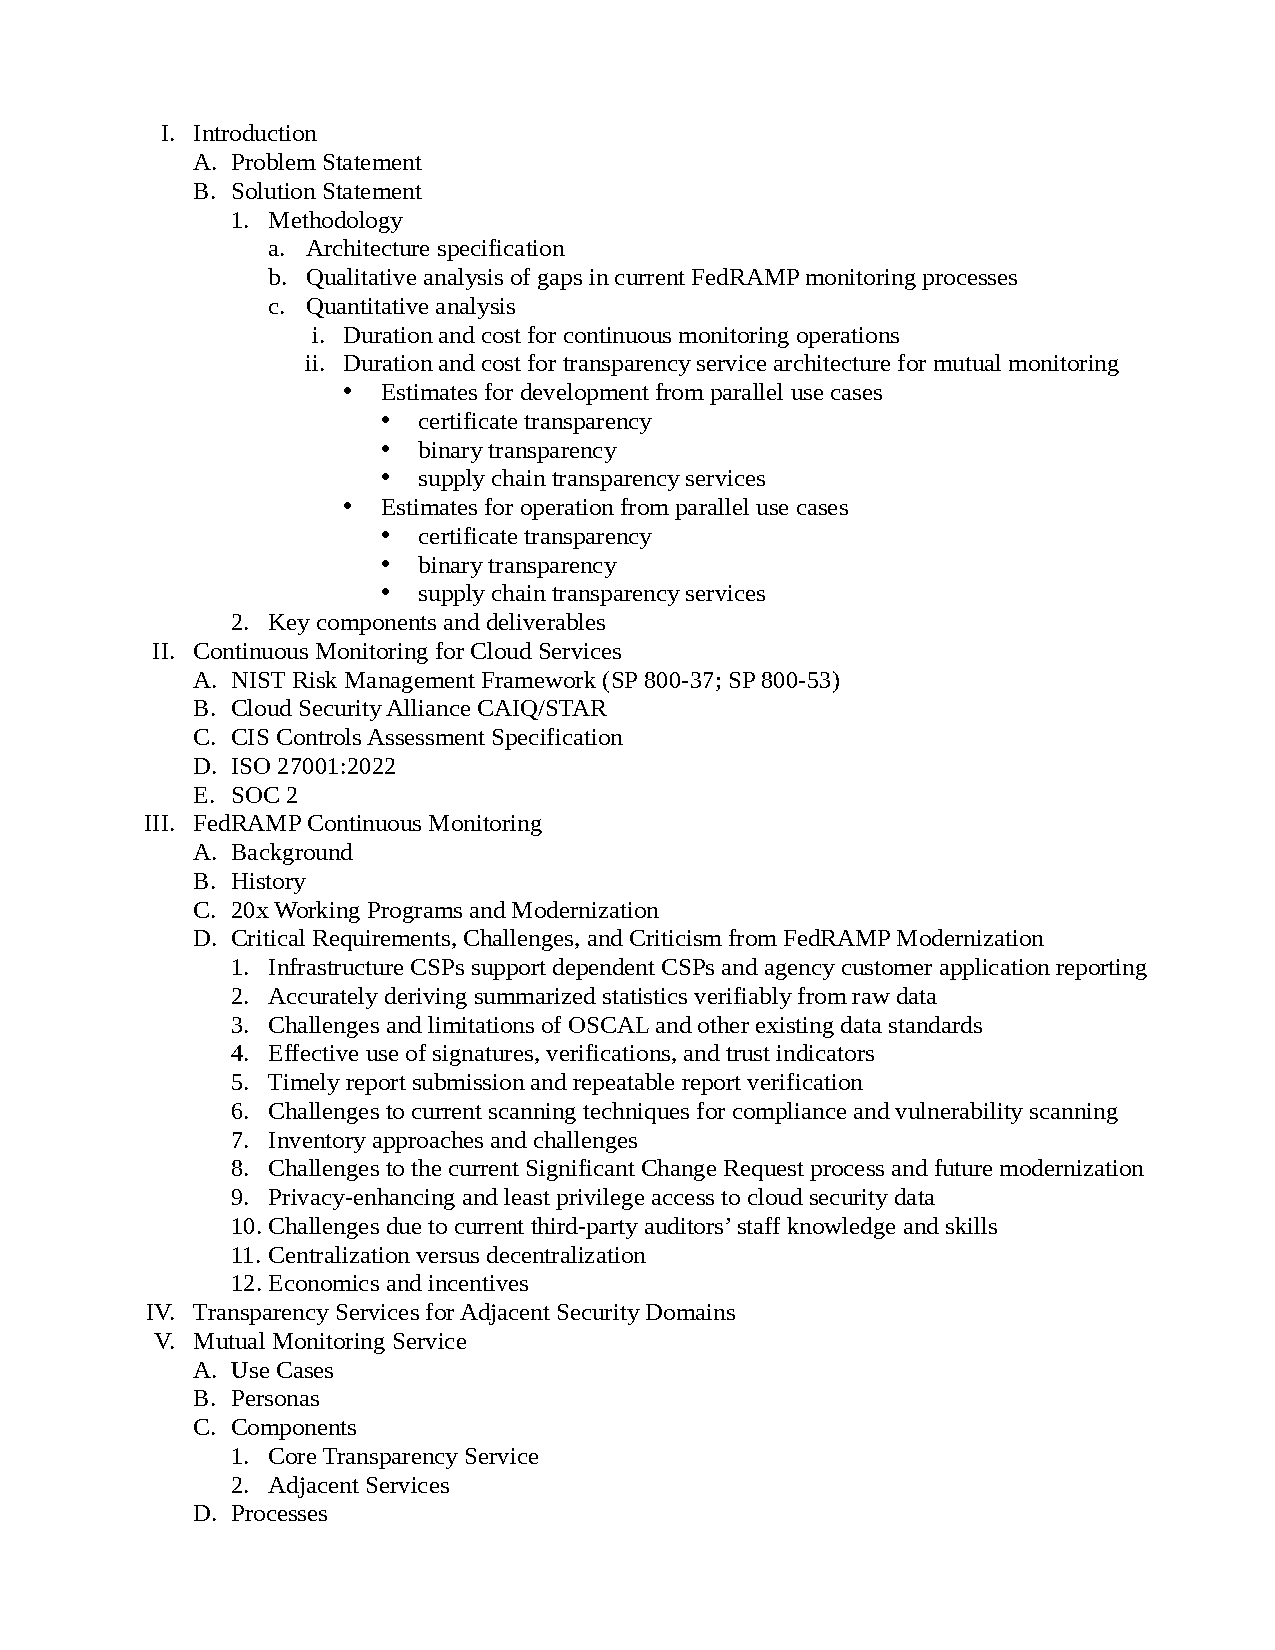
\includepdf[pages=-]{outline.pdf}

\nocite{*}
\bibliographystyle{apacite}
%  Relatives path work because you initialize top-level practicum repo
%  so the paths are consistent. Clone this repo and initialize the
%  submodules and it will work.
%  https://github.com/aj-stein/practicum.git
\bibliography{../references.bib}

\section*{\centering{Appendix}}

%  Relatives path work because you initialize top-level practicum repo
%  so the paths are consistent. Clone this repo and initialize the
%  submodules and it will work.
%  https://github.com/aj-stein/practicum.git
\includepdf[pages=-]{../prototype/build/architecture.pdf}

\end{document}
